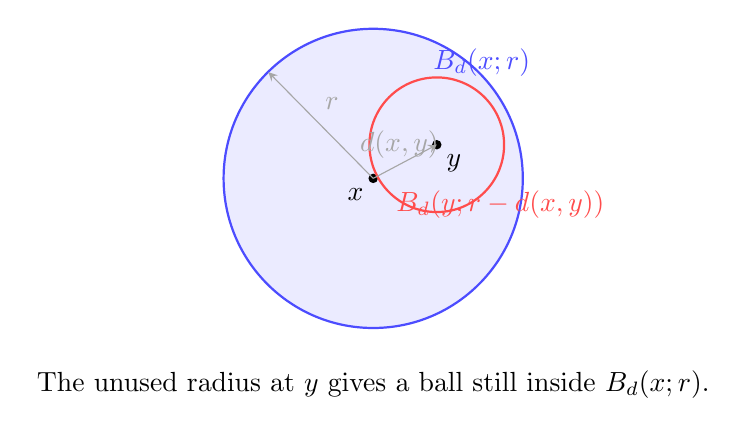
\begin{tikzpicture}[scale=0.95,>=stealth]
  \fill[blue!8] (0,0) circle (2.0);
  \draw[blue!70,thick] (0,0) circle (2.0);
  \node[blue!70] at (1.45,1.55) {\(B_d(x;r)\)};

  \fill[black] (0,0) circle (1.8pt);
  \node[below left] at (0,0) {\(x\)};

  \coordinate (y) at (0.85,0.45);
  \fill[black] (y) circle (1.8pt);
  \node[below right] at (y) {\(y\)};

  \draw[red!70,thick] (y) circle (0.9);
  \node[red!70] at (1.7,-0.35) {\(B_d(y;r-d(x,y))\)};

  \draw[->,gray!70] (0,0) -- (y);
  \node[gray!70] at (0.35,0.45) {\(d(x,y)\)};
  \draw[->,gray!70] (0,0) -- (-1.4,1.42);
  \node[gray!70] at (-0.55,1.0) {\(r\)};

  \node[align=center] at (0,-2.75)
    {The unused radius at \(y\) gives a ball still inside \(B_d(x;r)\).};
\end{tikzpicture}
